\documentclass[11pt]{article}
\usepackage[margin=1.05in]{geometry}
\usepackage{amsmath,amssymb,amsthm}
\usepackage{booktabs}
\usepackage{array}
\usepackage{tabularx}
\usepackage[protrusion=true,expansion=false]{microtype}
\usepackage[table]{xcolor}
\usepackage{enumitem}
\usepackage{titlesec}
\usepackage{float}
\usepackage{tikz}
\usetikzlibrary{arrows.meta,positioning,calc,backgrounds}
\usepackage{hyperref}

\hypersetup{colorlinks=true, linkcolor=blue!60!black, urlcolor=blue!60!black, citecolor=blue!60!black}
\usepackage[skip=0.6\baselineskip, indent=0pt]{parskip}

\titleformat{\section}{\large\bfseries}{\thesection.}{0.7em}{}
\titleformat{\subsection}{\normalsize\bfseries}{\thesubsection.}{0.6em}{}

\theoremstyle{plain}
\newtheorem{proposition}{Proposition}
\theoremstyle{definition}
\newtheorem{definition}{Definition}

% ----- notation -----
\newcommand{\vmax}{V_{\max}}
\newcommand{\Tc}{T_{\mathrm{close}}}
\newcommand{\bcorr}{b_{\mathrm{corr}}}
\newcommand{\tx}[1]{\texttt{#1}}
\newcommand{\be}[2]{\langle #1\rangle_{#2}}
\newcommand{\pre}[2]{[#1]_{#2}}
\newcommand{\xo}[1]{\mathsf{x}(#1)}
\newcommand{\Ht}[1]{H_{\textsf{#1}}}
\newcommand{\Hb}[1]{H^{\mathrm{B}}_{\textsf{#1}}}
\newcommand{\Sign}{\mathsf{Sign}}
\newcommand{\Vfy}{\mathsf{Verify}}
\newcommand{\PSign}{\mathsf{PreSign}}
\newcommand{\PVfy}{\mathsf{PreVerify}}
\newcommand{\Compl}{\mathsf{Complete}}
\newcommand{\Extr}{\mathsf{Extract}}
\newcommand{\Wots}{\mathsf{W}}
\newcommand{\kiss}{k_{\mathrm{iss}}}
\newcommand{\Piss}{P_{\mathrm{iss}}}
\newcommand{\owed}{\mathsf{owed}}
\newcommand{\PH}{P_H^{c}}
\newcommand{\Oc}{O_c}
\newcommand{\KQ}{K_{Q}^{c}}
\newcommand{\Kb}{K_{b}^{c}}
\newcommand{\Kcorr}{K_{\mathrm{corr}}^{c}}
\newcommand{\KU}{K_{U}^{c}}
\newcommand{\Acorr}{A_{\mathrm{corr}}^{c}}
\newcommand{\AU}{A_{U}^{c}}
\newcommand{\kin}{k_{\mathrm{in}}}
\newcommand{\vin}{v_{\mathrm{in}}}
\newcommand{\vout}{v_{\mathrm{out}}}

\newcolumntype{L}{>{\raggedright\arraybackslash}X}
\renewcommand{\arraystretch}{1.3}
\makeatletter
\setlength{\@fptop}{0pt}
\setlength{\@fpsep}{1.5\baselineskip}
\setlength{\@fpbot}{0pt plus 1fil}
\makeatother

\newenvironment{algobox}[1]
  {\par\smallskip\noindent\begin{tabular}{|p{0.955\linewidth}|}\hline\textbf{#1}\\[2pt]}
  {\\\hline\end{tabular}\par\smallskip}

\title{\textbf{The grants L2}\\a Lichen L2 without global order\\[2pt]\large early draft: one note per account, in sequence}
\author{waxwing}
\date{Version 0.5, November 2026\\[2pt]\small a companion to \emph{Lichen}, version 0.5~\cite{lichen}}

\begin{document}
\maketitle

\begin{abstract}
The grants L2 is a Lichen L2 with no global order: no sequencer, no
anchoring, and no ledger but the hub's book. A user's contract locks her
deposit with the hub's liquidity on Bitcoin, and her exit is judged
only on evidence she signed.

Each key is an \emph{account}, holding exactly one note at a time,
numbered in sequence: $(o, k, v)$, owner, sequence number, value. A
payment is a \emph{joint spend} that moves the payer's account and the
payee's one step each, and both sign it; one grant from the hub opens
both new notes, so the payment completes for both or for neither. The
payee must be online to be paid, like a Lightning payee. Each account is
ordered and the system is not, and the order within an account does the
rest.

A claim is one note, 74 bytes on chain. The hub answers any claim by
citing one spend: a later step of the same account supersedes the
claimed note, so a spend in flight needs no naming, and a stale claim
never pays more than a current one. The algorithm that judges an exit is
one comparison of sequence numbers. The hub stores $O(1)$ per account,
its latest step, so $O(N)$ for $N$ users however many payments they
make; the user stores only her live note. Since nothing is kept per
payment, an account can make billions of payments on a 32-bit counter:
volume is limited by rate, not storage (\S\ref{sec:volume-pay}). Every
balance is claimable in full, so none of it is left at the hub's mercy.
Notes are signed with BIP340 and encrypted by adaptor, and the hub's
statement needs no pairing: about 1.7M cycles (estimated). A deferred
receipt through a mailbox is set apart as an option
(\S\ref{sec:deferred}), and \S\ref{sec:compare} compares the design with
version 0.4, which lets a key hold many notes. A proposal; nothing here
is built.
\end{abstract}

\tableofcontents

\section{Setting}\label{sec:setting}

A Lichen contract (\cite{lichen}, \S3) locks the hub's liquidity and the
user's deposit in one Bitcoin output, with a cap $\vmax$, reserves $r_A$
(hers) and $r_H$ (the hub's), and a close time $\Tc$. Amounts on chain
are counted in the contract's \emph{unit} $u$ (sats per unit): an amount
$b$ is a 4-byte word, paid out as $u\,b$ sats. It ends in one of three
ways:
\begin{itemize}[nosep]
\item \textbf{Fold}: both sign; the user is paid what she withdraws and
  her reserve.
\item \textbf{Default}: after $\Tc$, the user is paid $r_A$ and the hub
  the rest. She must withdraw or exit before.
\item \textbf{Exit}: the user posts \tx{request} with a claim of $b$
  units; she is paid $b$, or the hub's correction $\bcorr \le b$ if the
  hub proves she is owed no more. The proof is checked by BABE, by which
  Alice can show a false proof without any key (\cite{lichen}).
\end{itemize}

The hub's book is the only ledger, and nothing is ordered across
accounts. What a global history would otherwise provide is \emph{evidence
the user signed}: a claim is reduced only by a spend she authorized and
whose unlock the hub publishes. Users need the chain only for that,
when something is stuck (\S\ref{sec:state}).

\textbf{Contracts and credit.} A user's participation is defined by her
contract. Contract $c$ has an L2 key $\Oc$ of its own, fresh at the
opening; the note of $\Oc$ is what $c$'s exit claims. A note under any
other key (a wallet with no contract, a closed contract's key) is the
hub's IOU with no backing on chain: credit.

\textbf{Accounts.} Each key is an \emph{account}: a sequence of notes,
numbered $0, 1, 2, \dots$, of which exactly one is live. Receiving is a
step of the receiver's account, so the receiver signs it. Accounts are
ordered one by one and not against each other: a payment advances two
accounts at once, and nothing relates Alice's numbers to Bob's.

\textbf{The hub checks amounts for itself.} Whatever the hub signs alone
(a note, a grant, a reissue) can only add to what it owes. It can lower
a user's balance only through a spend she signed. So the checks on
amounts that the hub makes when it records a payment, such as whether
the payer's loss equals the payee's gain, protect only the hub, and
nothing else enforces them. If it lets a party gain too much, it prints
money at its own expense: it has signed that note. If it gives a party
too little, that party doesn't sign. The statement that judges an exit
(\S\ref{sec:statement}) never checks that a payment balances.

\section{Notation}\label{sec:notation}

\subsection{Group, encodings, hashes}

\begin{itemize}[nosep]
\item secp256k1: generator $G$, group order $n$. It carries Bitcoin's
  keys, the L2's owner keys and the issuer's key.
\item Lower-case letters are scalars, upper-case letters points.
\item $\xo{P}$: the 32-byte x-coordinate of $P$. $\mathsf{lift}(x)$: the
  point with x-coordinate $x$ and even $y$. $P^{(33)}$: $P$ compressed.
\item Every public key is x-only (BIP340~\cite{bip340}): a key pair $(d,
  P)$ has $P = dG$ with even $y$, $d$ negated if needed.
\item $\be{v}{k}$: $v$ as $k$ bytes, big-endian. $\pre{h}{k}$: the first
  $k$ bytes of $h$. $\|$: concatenation.
\item $\Ht{tag}(p_1, \dots, p_r)$, the L2's tagged hash:
  \[
    \mathrm{SHA256}\big(\textsf{tag} \,\|\, \texttt{0x00} \,\|\, \be{|p_1|}{4}
    \,\|\, p_1 \,\|\, \cdots \,\|\, \be{|p_r|}{4} \,\|\, p_r\big),
  \]
  with the tags \textsf{note}, \textsf{half}, \textsf{spend},
  \textsf{auth}, \textsf{unlock} and \textsf{unlock-scalar}, each
  prefixed \textsf{lichen/notes/}, written $\Ht{note}, \Ht{half},
  \dots$. Every part is length-prefixed, so no two
  different part lists hash alike.
\item $\Hb{tag}(x) = \mathrm{SHA256}(\mathrm{SHA256}(\textsf{tag}) \,\|\,
  \mathrm{SHA256}(\textsf{tag}) \,\|\, x)$, and BIP340's challenge $e(R,
  P, m) = \Hb{BIP0340/challenge}(\xo{R} \,\|\, \xo{P} \,\|\, m) \bmod n$,
  which depends on $R$ only through $\xo{R}$.
\end{itemize}

\subsection{Signatures}

\textbf{BIP340.} $\Sign_d(m) = (r, s)$ with $r = \xo{R}$, $R = kG$ of
even $y$, $s = k + e(R, P, m)\,d$; 64 bytes. $\Vfy_P(m, (r, s))$ holds
iff $sG = \mathsf{lift}(r) + e(\mathsf{lift}(r), P, m)P$. An owner's
signature on a spend is written $\psi$, the issuer's on a note
$\sigma$.

\textbf{Adaptor signatures}~\cite{poelstra,aumayr}. For a point $T =
tG$, the issuer's pre-signature on $m$ is $\rho = \PSign_{\kiss}(m, T) =
(R', s')$: it draws $k$ until $R = kG + T$ has even $y$, sets $R' = kG$
and $s' = k + e(R, \Piss, m)\,\kiss$. $\PVfy_{\Piss}(m, T, \rho)$ holds
iff $s'G = R' + e(R' + T, \Piss, m)\Piss$ and $R' + T$ has even $y$.
$\Compl(\rho, t) = (\xo{R' + T},\ s' + t)$ is an ordinary BIP340
signature on $m$, and $\Extr(\sigma, \rho) = s - s'$ gives $t$ back. A
pre-signature is 65 bytes ($R'$ compressed, $s'$). The design never
needs to extract: $t$ always travels in the clear (\S\ref{sec:payment},
\S\ref{sec:correct}).

Notes are signed with BIP340 because a claim holds one note, so nothing
needs aggregating, and because the statement then verifies BIP340, which
RISC Zero accelerates.

\textbf{One-time signatures.} $\Wots_K(x)$ is a Winternitz signature
under the one-time key $K$ on the bytes $x$: 4-bit digits (2 a byte)
plus checksum digits, each digit given as 2 witness items (a hash
preimage and the digit itself). The chains are SHA-256 for Alice's keys,
which the statement verifies (RISC Zero accelerates SHA-256), and
HASH160 for the hub's, which only script reads. Script verifies it digit
by digit, so the digits on the stack are authenticated by the
signature, and script can compare them with other digits. A key fixed
in a leaf at the opening signs once; two different signatures under it
are an \emph{equivocation}, which some leaves punish (\S\ref{sec:bits}).

\subsection{Keys}

\begin{center}
\begin{tabularx}{\linewidth}{llL}
\toprule
Symbol & Scope & Use \\
\midrule
$\kiss$, $\Piss = \kiss G$ & the deployment (one) & the issuer's key: signs every note; pre-signs every grant's new notes \\
$\PH$ & contract $c$ & the hub's payment key: its half of the 2-of-2 on every link of $c$'s graph \\
$P_A^c$ & contract $c$ & her half of the 2-of-2 \\
$a_c$, $\Oc = a_cG$ & contract $c$ & her L2 key, fresh for $c$: owns $c$'s account; signs its steps \\
$\KQ$, $\Kb$ & contract $c$, hers & one-time: the posted claim $Q$ and $b$, in \tx{request} \\
$\Kcorr$, $\KU$ & contract $c$, the hub's & one-time: $\bcorr$ and the unlock $U$, in \tx{correct} \\
$\Acorr$, $\AU$ & contract $c$, hers & one-time: her countersignatures on $\bcorr$ and $U$, in \tx{ack} \\
$z_S$, $t_S$, $T_S = t_S G$ & spend $S$ & the spend's unlock: a 16-byte seed, its scalar, its point \\
\bottomrule
\end{tabularx}
\end{center}

The hub derives each contract's keys from its seed and $c$, and $\kiss$
once: $\Piss$ is common to every contract. Alice derives hers from her
wallet's key and the contract's nonce.

\section{Accounts, spends and grants}

\subsection{Notes}\label{sec:notes}

\begin{definition}
A \emph{note} is $N = (o, k, v)$: an owner, a sequence number $0 \le k <
2^{32}$, and a value $0 \le v < 2^{48}$ sats. Its digest is $\delta(N) =
\Ht{note}(o, \be{k}{4}, \be{v}{6})$. It is \emph{settled} when its
holder has $\sigma_N = \Sign_{\kiss}(\delta(N))$.
\end{definition}

\textbf{Values are in sats, 6 bytes.} Every value in the L2 is $v <
2^{48}$ sats and is encoded in 6 bytes, in digests and on chain alike.
The unit $u$ applies only to the amounts $b$ paid out on chain, so
$u\,b \le v < 2^{48} = 2^{32} \cdot 2^{16}$: six bytes cover every
payout of a 4-byte $b$ for any unit up to 65,536 sats. Payments below a
unit are ordinary payments; rounding happens once, at exit.

\textbf{Every account starts at 0.} A contract key's note 0 is its
\emph{mint}, $(\Oc, 0, v_0)$, which the contract vouches for
(\S\ref{sec:opening}); any other key's note 0 is the empty note $(o, 0,
0)$. Neither needs a signature. Each spend an account takes part in
moves it from $k$ to $k + 1$. A value may be 0: a payer who spends her
whole balance keeps a note of 0, and her account goes on.

\textbf{Names.} A note is named by its owner and number, which are
unique as long as each account has one live note. Numbers are assigned
by the account's history, not chosen by anyone, so nothing else needs
an identifier.

\textbf{The invariant: one live note per account.} The hub keeps it by
recording a spend only if it takes each owner's live note; the owner
keeps it by signing only spends of the note she holds (Rule 3,
\S\ref{sec:rules}).

\subsection{Spends, in halves}\label{sec:spend}

\begin{definition}
A \emph{half} for owner $o$ is $\eta = (o,\ \kin,\ \vin,\ \vout,\
\lambda)$: $o$'s note $(o, \kin, \vin)$, the value $\vout$ it leaves
with, and a 16-byte blinding $\lambda$ that $o$ chooses. Its digest is
\[
  h(\eta) = \Ht{half}\big(o,\ \be{\kin}{4},\ \be{\vin}{6},\
  \be{\vout}{6},\ \lambda\big),
\]
and its \emph{step} gives $o$ the note $(o, \kin + 1, \vout)$.

A \emph{spend} $S$ is two halves with distinct owners, $o_1 < o_2$ as
bytes. Its digest, the message both owners approve, is
\[
  \delta(S) = \Ht{spend}\big(o_1,\ h(\eta_1),\ o_2,\ h(\eta_2)\big).
\]
The hub records a spend only if it is \emph{well formed}: each half's
note is its owner's live one, and $v_{\mathrm{in},1} + v_{\mathrm{in},2}
= v_{\mathrm{out},1} + v_{\mathrm{out},2}$.
\end{definition}

The second condition is the hub's own (\S\ref{sec:setting}): nothing
else checks it, and a hub that broke it would only pay more than it took
in.

$\delta(S)$ is a hash of the spend's contents, as any signed message is
hashed. It is not an identifier: no note records it, no claim posts it,
and nothing refers to it. A spend is named, if it needs naming, by the
two notes it takes, $(o_1, k_1)$ and $(o_2, k_2)$: each note is taken
once, so the pair is unique.

\textbf{Why the owners appear twice.} In $\delta(S)$ they are in the
clear, because two checks need the counterparty's key while seeing only
its half's digest. The statement verifies the other owner's signature
under the key that Alice approved (Rule 1, \S\ref{sec:rules}): were the
key only inside $h(\eta_2)$, the hub could supply a key of its own and a
signature to match. And a payer checks that the payee is the one on her
invoice. Inside $h(\eta)$, each half names its own owner, so a half
means the same whatever it is embedded in.

A payment of $a$ from Alice, holding $(o_A, k_A, v_A)$, to Bob, holding
$(o_B, k_B, v_B)$, has the halves $(o_A, k_A, v_A, v_A - a, \lambda_A)$
and $(o_B, k_B, v_B, v_B + a, \lambda_B)$.

\textbf{Halves hide balances from the counterparty.} Each party sees
its own half and the other's digest. Both know $a$; neither learns the
other's balance or number. The blinding keeps the digest from being
searched by anyone who knows the owner and could guess the values. The
hub sees both halves.

\subsection{Grants}\label{sec:grant}

\begin{definition}
The hub's \emph{grant} on a well-formed spend $S$ is $\Gamma = (T_S,\
\rho_1,\ \rho_2)$, with
\begin{gather*}
  z_S = \pre{\Ht{unlock}(\kiss, \delta(S))}{16},\qquad T_S = t_S G,\\
  t_S = \Ht{unlock-scalar}(z_S, \be{\mathit{ctr}}{4})\ \ (\text{the least
  } \mathit{ctr} \text{ with } 0 < t_S < n),\\
  \rho_i = \PSign_{\kiss}\big(\delta(o_i, k_{\mathrm{in},i} + 1,
  v_{\mathrm{out},i}),\ T_S\big),\qquad i = 1, 2,
\end{gather*}
the pre-signatures on the two new notes. The message both owners sign is
\[
  \alpha = \Ht{auth}\big(\delta(S),\ T_S^{(33)},\ \rho_1^{(65)},\
  \rho_2^{(65)}\big).
\]
\end{definition}

Each owner checks the pre-signature on its own new note and signs
$\alpha$, which covers the other's as bytes. So both sign one grant:
the same $T_S$, and so the same unlock, opens both new notes. The seed
$z_S$ is derived from the spend, so the hub keeps no secret per spend.

\section{A payment}\label{sec:payment}

\subsection{Live receipt}\label{sec:live}

Figure~\ref{fig:payment}. Bob gives Alice an invoice $(o_B, a)$; both
are online.

\begin{figure}[!tbp]
\centering
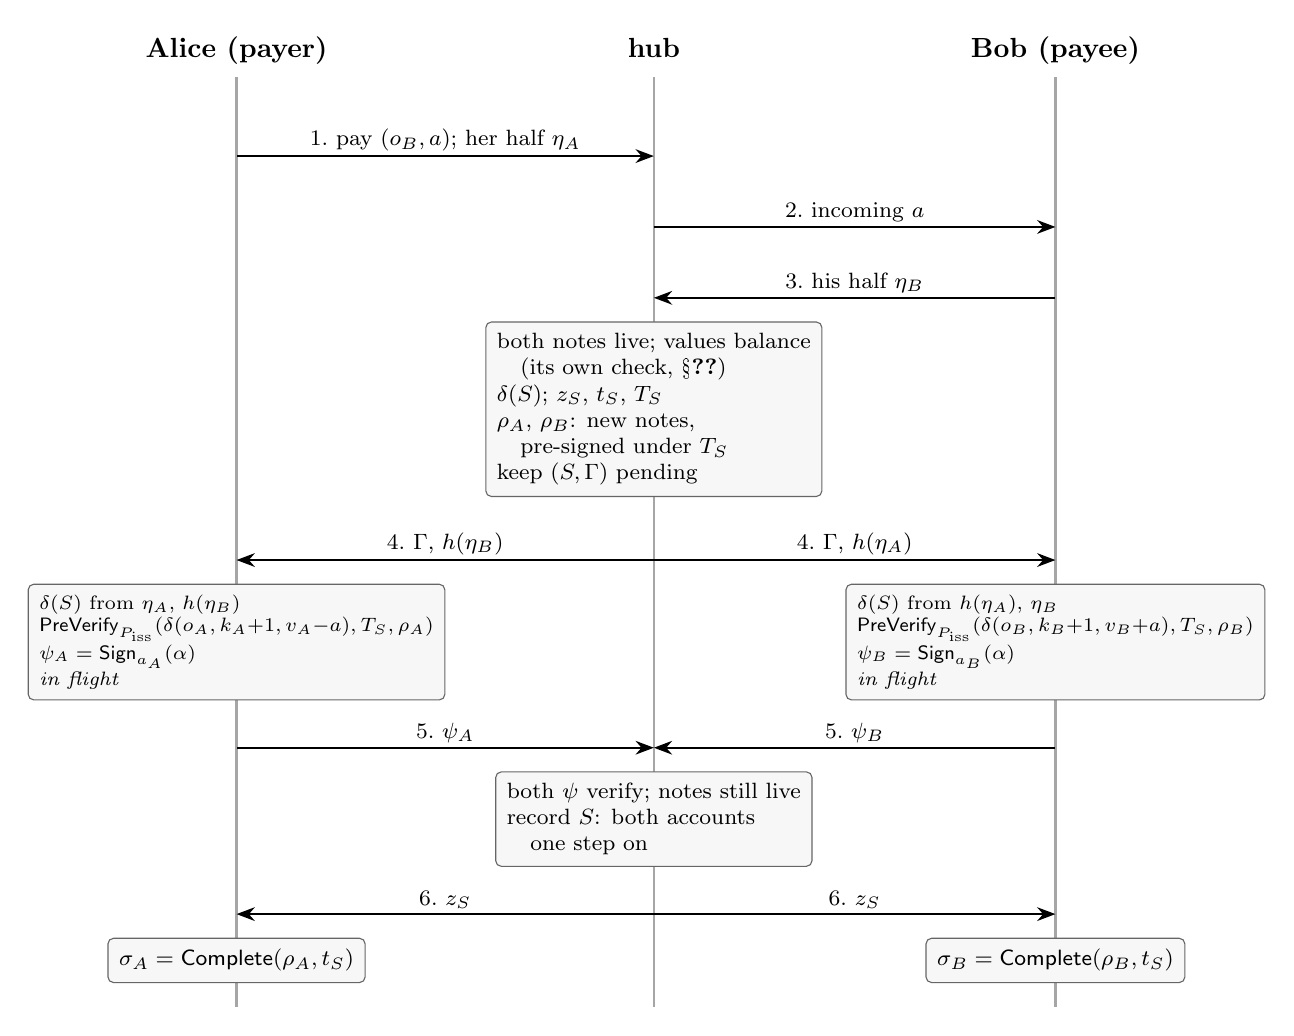
\begin{tikzpicture}[>=Stealth, font=\small,
  life/.style={draw=black!35, thick},
  box/.style={draw=black!60, fill=black!3, rounded corners=2pt, align=left, inner sep=4pt, font=\footnotesize},
  msg/.style={->, thick},
  lbl/.style={align=center, font=\footnotesize, inner sep=1.5pt}]
\coordinate (LA) at (2.7,0); \coordinate (LH) at (8.0,0); \coordinate (LB) at (13.1,0);
\node[font=\bfseries, anchor=base] at ($(LA)+(0,0.25)$) {Alice (payer)};
\node[font=\bfseries, anchor=base] at ($(LH)+(0,0.25)$) {hub};
\node[font=\bfseries, anchor=base] at ($(LB)+(0,0.25)$) {Bob (payee)};
\coordinate (y) at (0,-1.0);
\draw[msg] (LA|-y) -- node[lbl, above] {1.\ pay $(o_B, a)$; her half $\eta_A$} (LH|-y);
\coordinate (y) at ($(y)+(0,-0.9)$);
\draw[msg] (LH|-y) -- node[lbl, above] {2.\ incoming $a$} (LB|-y);
\coordinate (y) at ($(y)+(0,-0.9)$);
\draw[msg] (LB|-y) -- node[lbl, above] {3.\ his half $\eta_B$} (LH|-y);
\node[box, anchor=north] (b1) at ($(LH|-y)+(0,-0.3)$) {
  both notes live; values balance\\ \quad (its own check, \S\ref{sec:setting})\\
  $\delta(S)$; $z_S$, $t_S$, $T_S$\\
  $\rho_A$, $\rho_B$: new notes,\\ \quad pre-signed under $T_S$\\
  keep $(S, \Gamma)$ pending};
\coordinate (y) at ($(b1.south)+(0,-0.8)$);
\draw[msg] (LH|-y) -- node[lbl, above] {4.\ $\Gamma$, $h(\eta_B)$} (LA|-y);
\draw[msg] (LH|-y) -- node[lbl, above] {4.\ $\Gamma$, $h(\eta_A)$} (LB|-y);
\node[box, anchor=north, font=\scriptsize] (b2) at ($(LA|-y)+(0,-0.3)$) {
  $\delta(S)$ from $\eta_A$, $h(\eta_B)$\\
  $\PVfy_{\Piss}(\delta(o_A, k_A{+}1, v_A{-}a), T_S, \rho_A)$\\
  $\psi_A = \Sign_{a_A}(\alpha)$\\
  \emph{in flight}};
\node[box, anchor=north, font=\scriptsize] (b3) at ($(LB|-y)+(0,-0.3)$) {
  $\delta(S)$ from $h(\eta_A)$, $\eta_B$\\
  $\PVfy_{\Piss}(\delta(o_B, k_B{+}1, v_B{+}a), T_S, \rho_B)$\\
  $\psi_B = \Sign_{a_B}(\alpha)$\\
  \emph{in flight}};
\coordinate (y) at ($(b2.south)+(0,-0.6)$);
\draw[msg] (LA|-y) -- node[lbl, above] {5.\ $\psi_A$} (LH|-y);
\draw[msg] (LB|-y) -- node[lbl, above] {5.\ $\psi_B$} (LH|-y);
\node[box, anchor=north] (b4) at ($(LH|-y)+(0,-0.3)$) {
  both $\psi$ verify; notes still live\\
  record $S$: both accounts\\ \quad one step on};
\coordinate (y) at ($(b4.south)+(0,-0.6)$);
\draw[msg] (LH|-y) -- node[lbl, above] {6.\ $z_S$} (LA|-y);
\draw[msg] (LH|-y) -- node[lbl, above] {6.\ $z_S$} (LB|-y);
\node[box, anchor=north] (b5) at ($(LA|-y)+(0,-0.3)$) {$\sigma_A = \Compl(\rho_A, t_S)$};
\node[box, anchor=north] (b6) at ($(LB|-y)+(0,-0.3)$) {$\sigma_B = \Compl(\rho_B, t_S)$};
\coordinate (end) at ($(b5.south)+(0,-0.3)$);
\begin{scope}[on background layer]
\foreach \l in {LA,LH,LB} \draw[life] (\l) -- (\l|-end);
\end{scope}
\end{tikzpicture}
\caption{A live payment: one step of each account. Each party is in
flight from its signature (step 5) until it has $z_S$ (step 6). Either
can hand $z_S$ to the other.}
\label{fig:payment}
\end{figure}

The payment is complete for a party when it holds $z_S$: its new note
is then settled. Alice's receipt is $z_S$; Bob's acceptance is his
$\psi_B$, which the hub can show her. Either party holding $z_S$ can
hand it to the other, so neither depends on the hub to learn that the
other side completed.

\textbf{In flight.} From its signature until it holds $z_S$, a party
keeps its old note and $(S, \Gamma)$. It needs nothing else. Its claim
names the old note, and if the hub uses $S$ against that claim, it must
publish $z_S$, and both new notes count. The claimant is owed her new
note's value: the hub's correction is $\bcorr = \lfloor \vout/u
\rfloor$, which it can prove (\S\ref{sec:algo}); she needs no signature
on the new note for that. The counterparty's new note settles from the
published seed, as in an atomic swap.

\subsection{Rules}\label{sec:rules}

Each rule is named by who enforces it: the statement, against the hub;
the wallet, for its owner. Nothing relies on the hub, which checks only
for itself (\S\ref{sec:setting}).

\textbf{Rule 1 (the statement): a spend counts only with both owners'
signatures, together.} Publishing $z_S$ settles a new note only for a
party that holds its pre-signature. Each $\psi$ is the statement's
evidence that its signer does: $\alpha$ commits to $T_S$, $\rho_1$ and
$\rho_2$, and a wallet signs only after checking its own $\rho$ and
keeping the grant. Without the rule, the hub could take $\psi_A$ alone,
cite $S$ against Alice and publish $z_S$, while Bob never received
$\rho_B$: Alice debited, Bob not credited, the step made one-sided. So a
cited spend is usable only if $\psi_1$ and $\psi_2$ both verify on
$\alpha$ (\S\ref{sec:statement}), never with each checked apart or with
the claimant's alone. Then $S$ counts against no one until both have
signed, and whichever exit publishes $z_S$ settles both new notes.

\textbf{Rule 2 (the wallet): one pending signature per account.} A
wallet never signs a spend while another it signed is pending. If Bob
signed two incoming payments that both take his note $k$, the hub could
complete both and count each against its payer, while Bob's account
moves to $k+1$ only once. The hub can't make a wallet break this rule.
It means one payment at a time per account, in either direction; an
honest hub tells a second payer \emph{busy, retry}.

\textbf{Rule 3 (the wallet): sign only steps from the note you hold.}
Each owner checks its half: $(o, \kin, \vin)$ is its live note, and
$\vout$ the value it expects. This is the owner's side of the check on
amounts (\S\ref{sec:setting}): a half that leaves her too little, she
doesn't sign. So the account's invariant is the owner's own, whatever
the hub does, and every spend she ever signs has $\kin$ at most her
current number.

\textbf{Cancelling.} A party in flight asks the hub to cancel. If the
hub holds both signatures, it answers with $z_S$: the payment is done.
Otherwise it \emph{reissues} the party's note one step on, $(o, k + 1,
v)$, the same value with $\sigma$, and refuses $S$ from then on. The
party holds the reissue and nothing in flight. If the hub completed $S$
anyway, $S$ takes note $k$, which is behind the reissue: it can't count
against a claim of the reissue (\S\ref{sec:algo}), and the hub has paid
the counterparty from nothing. So a reissue needs no certificate: it is
just the account's next note. Like anything the hub signs alone, it can
only add: were it short, she would claim note $k$ instead, where the
worst the hub can cite is $S$, which she signed.

\subsection{What atomicity means here}\label{sec:atomic}

Once both have signed, the hub may record $S$ or not.
\begin{itemize}[nosep]
\item Not recorded, or cancelled: the hub alone knows $t_S$; the new
  notes never settle, and the old ones (or their reissues) stand.
\item Recorded, $z_S$ given to either party: both are paid, since the
  other can be handed $z_S$.
\item Recorded, $z_S$ withheld from both: both are in flight, and
  neither exit can be reduced through $S$ without publishing $z_S$,
  which settles both new notes.
\end{itemize}
So both parties are protected the same way: each one's step counts only
if the other's does.

\textbf{Evidence of payment.} A payee without $z_S$ has not been paid,
and delivers nothing. A payer debited for $S$ always holds $z_S$: she
gets it at step 6, or, if the hub counts $S$ against her at exit, from
its \tx{correct}, since citing $S$ means publishing its seed. She also
holds $\rho_B$, a part of the grant she signed. So whenever she has
paid, she can complete Bob's note herself by handing him $z_S$.

\textbf{Settling into a closed contract.} What can still go wrong is
timing: $z_S$ may reach Bob only after his contract has closed, when his
new note is credit. A hub can arrange it by withholding $z_S$ until Bob
has exited, then citing $S$ at Alice's exit: it keeps $a$. Two wallet
timeouts, set against the dispute's windows, close this. Let $c$ be the
time for a \tx{request} to confirm.
\begin{itemize}[nosep]
\item \textbf{The payer's, $p$.} A wallet in flight for longer than $p$
  exits. The hub must then decide on $S$ within $w_H$: publish $z_S$ in
  \tx{correct}, or never count $S$ against her, since her account
  closes at its old balance.
\item \textbf{The payee's, $L$.} A wallet signs no incoming payment
  after $\Tc - L$, with $L > p + w_H + 2c$, and doesn't withdraw or exit
  while an incoming payment is pending unless $\Tc - c$ forces it.
\end{itemize}
Then every payment Bob accepted is decided while his contract is open,
with time left to claim the new note. Choosing $p$ and $L$ is a
practical matter: $p$ trades a payer's patience with a slow hub against
exits, $L$ shortens the time a contract can receive, and an invoice can
carry the payee's last day for receiving. A payee colluding with the
hub harms only the two of them: the payer is debited only when $z_S$
exists, and $z_S$ completes the payee's note.

\section{The contract}\label{sec:contract}

\subsection{Opening}\label{sec:opening}

The opening follows~\cite{lichen} (Figure~\ref{fig:opening}). Her
deposit becomes an L2 balance through the \emph{mint}, note 0 of her
account, which the contract itself vouches for:
\begin{enumerate}[nosep]
\item Alice derives a fresh key $a_c$, $\Oc = a_cG$, and pays her
  deposit $v_D$ to a coin $O_D$: a 2-of-2 of hers and the hub's, or her
  refund alone after a timeout.
\item She asks for a contract with owner $\Oc$. The hub refuses an $\Oc$
  it has seen before, as the owner of a contract or of any account that
  has moved, so the account is new.
\item The setup (\cite{lichen}): the statement fixed by its journal $J$
  (\S\ref{sec:journal}), which binds her one-time keys and the mint's
  value $v_0$, her deposit less the opening's fee; the BABE instances
  garbled by Alice and kept by the hub by cut-and-choose.
\item The hub's offer: the funding $F$, spending $O_D$ and the hub's
  coins into the contract output, and its pre-signatures on the graph.
\item Alice signs the graph and $F$'s spend of $O_D$.
\item The hub adds its signature and broadcasts $F$.
\end{enumerate}
\textbf{The mint} $(\Oc, 0, v_0)$ has no signature: its evidence is the
contract, whose journal binds $v_0$. The hub enters it in its book once
$F$ confirms, and her spends of it are granted like any other. So the
swap is atomic by the contract's existence: if $F$ confirms, the
contract exists and the mint with it; if it never confirms, there is
neither, and Alice refunds $O_D$ after its timeout. A lost answer from
the hub costs her nothing: $F$ on chain is enough. The hub must not
record a spend of the mint before $F$ confirms, which is its own risk.

\begin{figure}[!tbp]
\centering
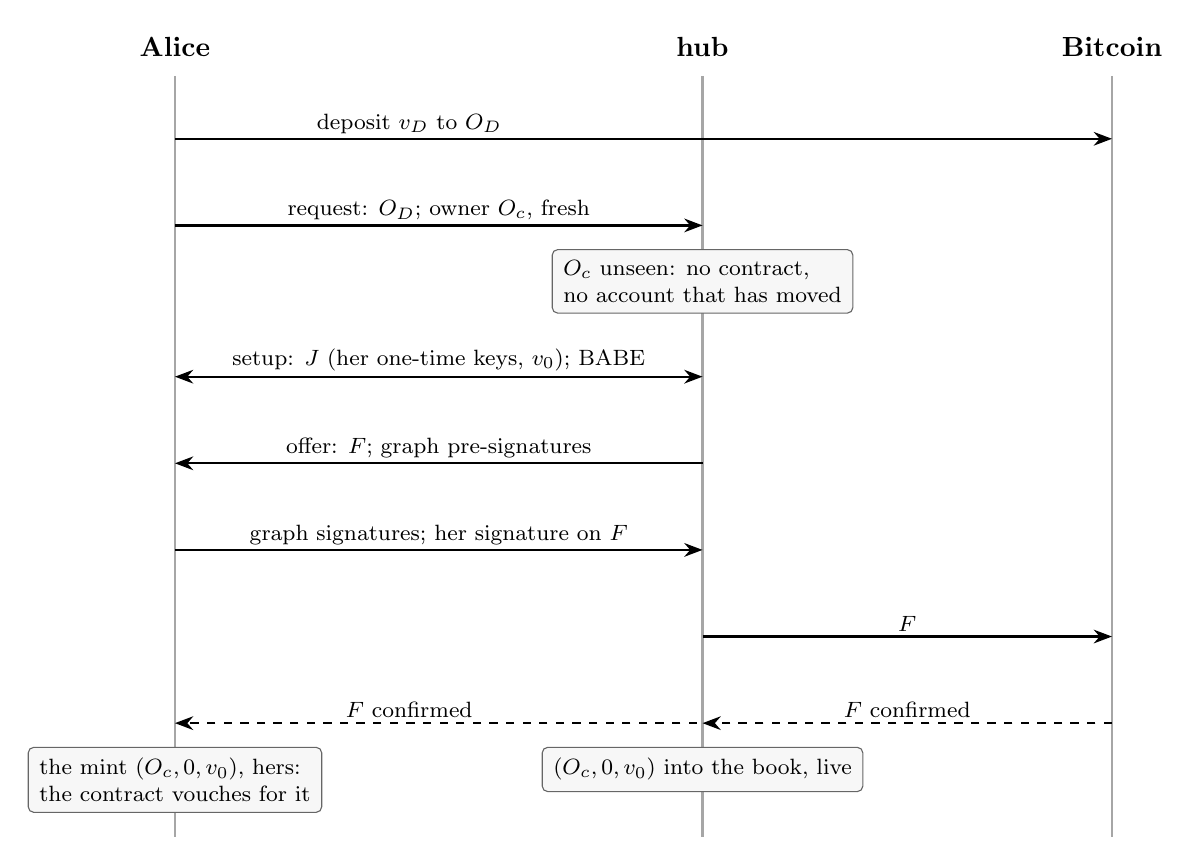
\begin{tikzpicture}[>=Stealth, font=\small,
  life/.style={draw=black!35, thick},
  box/.style={draw=black!60, fill=black!3, rounded corners=2pt, align=left, inner sep=4pt, font=\footnotesize},
  msg/.style={->, thick},
  lbl/.style={align=center, font=\footnotesize, inner sep=1.5pt}]
\coordinate (LA) at (2.6,0); \coordinate (LH) at (9.3,0); \coordinate (LB) at (14.5,0);
\node[font=\bfseries, anchor=base] at ($(LA)+(0,0.25)$) {Alice};
\node[font=\bfseries, anchor=base] at ($(LH)+(0,0.25)$) {hub};
\node[font=\bfseries, anchor=base] at ($(LB)+(0,0.25)$) {Bitcoin};
\coordinate (y) at (0,-0.8);
\draw[msg] (LA|-y) -- node[lbl, above, pos=0.25] {deposit $v_D$ to $O_D$} (LB|-y);
\coordinate (y) at ($(y)+(0,-1.1)$);
\draw[msg] (LA|-y) -- node[lbl, above] {request: $O_D$; owner $\Oc$, fresh} (LH|-y);
\node[box, anchor=north] (b1) at ($(LH|-y)+(0,-0.3)$) {$\Oc$ unseen: no contract,\\ no account that has moved};
\coordinate (y) at ($(b1.south)+(0,-0.8)$);
\draw[msg, <->] (LA|-y) -- node[lbl, above] {setup: $J$ (her one-time keys, $v_0$); BABE} (LH|-y);
\coordinate (y) at ($(y)+(0,-1.1)$);
\draw[msg] (LH|-y) -- node[lbl, above] {offer: $F$; graph pre-signatures} (LA|-y);
\coordinate (y) at ($(y)+(0,-1.1)$);
\draw[msg] (LA|-y) -- node[lbl, above] {graph signatures; her signature on $F$} (LH|-y);
\coordinate (y) at ($(y)+(0,-1.1)$);
\draw[msg] (LH|-y) -- node[lbl, above] {$F$} (LB|-y);
\coordinate (y) at ($(y)+(0,-1.1)$);
\draw[msg, dashed] (LB|-y) -- node[lbl, above] {$F$ confirmed} (LH|-y);
\node[box, anchor=north] (b3) at ($(LH|-y)+(0,-0.3)$) {$(\Oc, 0, v_0)$ into the book, live};
\draw[msg, dashed] (LB|-y) -- node[lbl, above, pos=0.75] {$F$ confirmed} (LA|-y);
\node[box, anchor=north] (b4) at ($(LA|-y)+(0,-0.3)$) {the mint $(\Oc, 0, v_0)$, hers:\\ the contract vouches for it};
\coordinate (end) at ($(b4.south)+(0,-0.3)$);
\begin{scope}[on background layer]
\foreach \l in {LA,LH,LB} \draw[life] (\l) -- (\l|-end);
\end{scope}
\end{tikzpicture}
\caption{The opening: the mint exists exactly when the contract does, so
the deposit and the L2 balance need no swap.}
\label{fig:opening}
\end{figure}

\subsection{The journal}\label{sec:journal}

The statement's only public input, fixed at the opening, is
\begin{align*}
  J &= \be{c}{4} \,\|\, D,\\
  D &= \mathrm{SHA256}\big(\texttt{"lichen/grants/contract"} \,\|\,
  \xo{\Piss} \,\|\, \xo{\Oc} \,\|\, \be{u}{8} \,\|\, \be{v_0}{6} \,\|\,
  \kappa\big),\\
  \kappa &= \mathrm{SHA256}\big(\KQ \,\|\, \Kb \,\|\, \Acorr \,\|\, \AU\big),
\end{align*}
$\kappa$ hashing Alice's four one-time public keys (each the list of its
chains' ends). $D$ binds the issuer, the owner, the unit, the mint's
value, and the keys under which every exit-time value reaches the
statement (\S\ref{sec:statement}). Without the owner, a hub could prove
against another key and call every claim malformed; without the unit,
it could prove at another $u$.

\subsection{The dispute graph}\label{sec:graph}

Every transaction has one input; every link has one output that carries
the value on, plus an anchor for fees. Each link is signed by the 2-of-2
$(P_A^c, \PH)$, pre-signed at the opening; each output has its
terminals. $\epsilon$ is a short relative lock on every link, so that a
link can't confirm in its parent's block. Figure~\ref{fig:graph} shows
the graph.

\begin{figure}[!tbp]
\centering
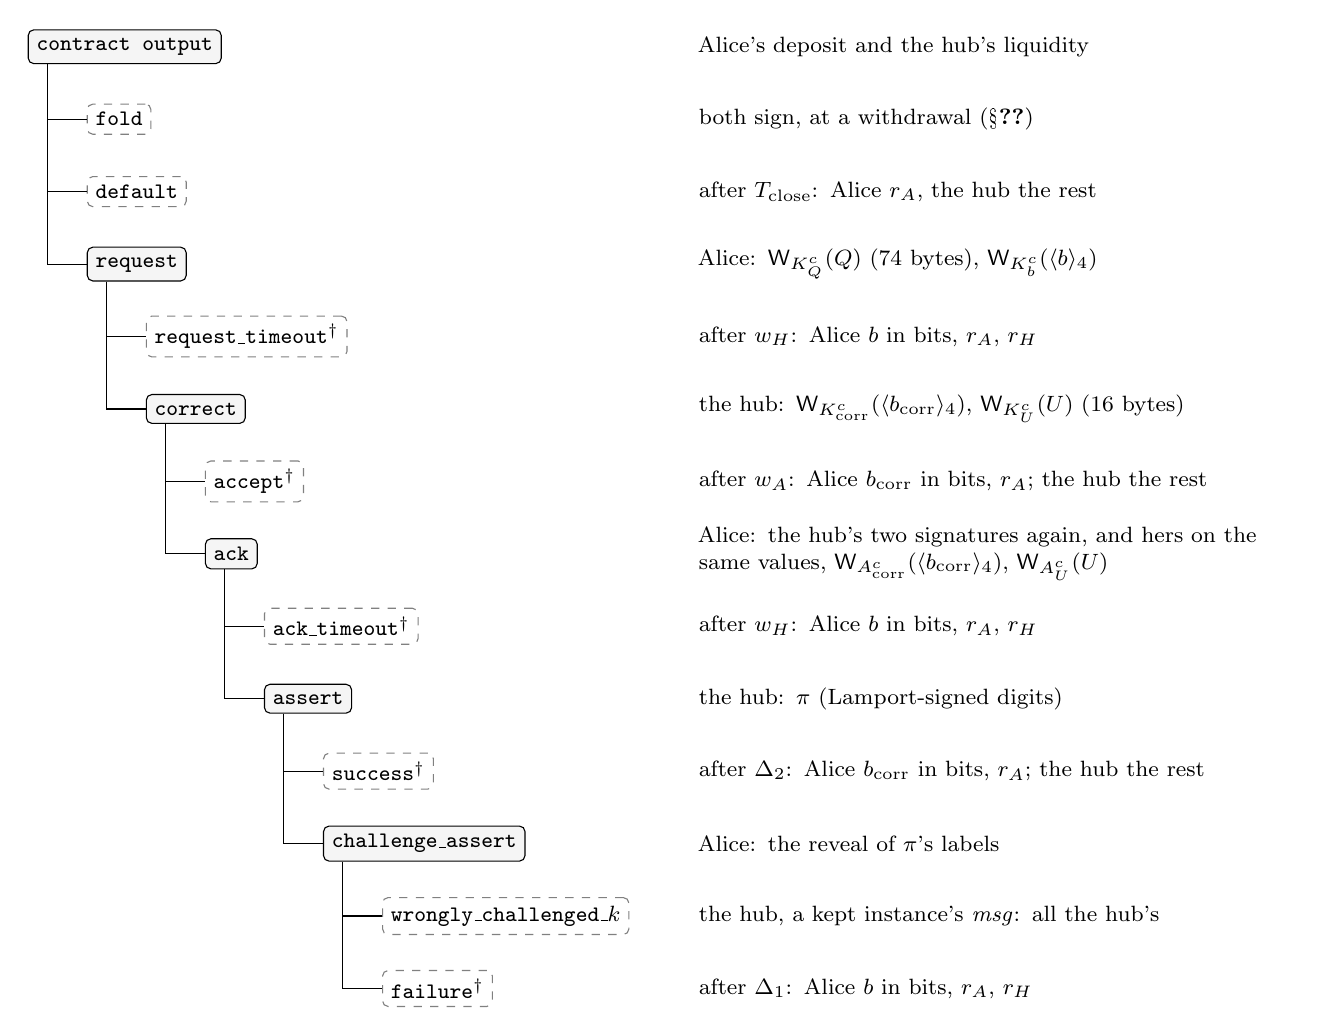
\begin{tikzpicture}[font=\footnotesize,
  link/.style={draw, rounded corners=2pt, inner sep=3pt, fill=black!4, font=\footnotesize\ttfamily, anchor=west},
  term/.style={draw=black!50, dashed, rounded corners=2pt, inner sep=3pt, font=\footnotesize\ttfamily, anchor=west},
  ann/.style={anchor=west, align=left, text width=7.5cm, font=\footnotesize}]
\def\dx{0.75}\def\dy{0.92}\def\ax{8.4}
\node[link] (c)  at (0*\dx, 0)       {contract output};
\node[term] (fo) at (1*\dx, -1*\dy)  {fold};
\node[term] (de) at (1*\dx, -2*\dy)  {default};
\node[link] (rq) at (1*\dx, -3*\dy)  {request};
\node[term] (rt) at (2*\dx, -4*\dy)  {request\_timeout$^\dagger$};
\node[link] (co) at (2*\dx, -5*\dy)  {correct};
\node[term] (ac) at (3*\dx, -6*\dy)  {accept$^\dagger$};
\node[link] (ak) at (3*\dx, -7*\dy)  {ack};
\node[term] (at) at (4*\dx, -8*\dy)  {ack\_timeout$^\dagger$};
\node[link] (as) at (4*\dx, -9*\dy)  {assert};
\node[term] (su) at (5*\dx, -10*\dy) {success$^\dagger$};
\node[link] (ch) at (5*\dx, -11*\dy) {challenge\_assert};
\node[term] (wc) at (6*\dx, -12*\dy) {wrongly\_challenged\_$k$};
\node[term] (fa) at (6*\dx, -13*\dy) {failure$^\dagger$};
\foreach \p/\q in {c/fo,c/de,c/rq,rq/rt,rq/co,co/ac,co/ak,ak/at,ak/as,as/su,as/ch,ch/wc,ch/fa}
  \draw ($(\p.south west)+(0.25,0)$) |- (\q.west);
\node[ann] at (\ax, 0)         {Alice's deposit and the hub's liquidity};
\node[ann] at (\ax, -1*\dy)    {both sign, at a withdrawal (\S\ref{sec:withdrawal})};
\node[ann] at (\ax, -2*\dy)    {after $\Tc$: Alice $r_A$, the hub the rest};
\node[ann] at (\ax, -3*\dy)    {Alice: $\Wots_{\KQ}(Q)$ (74 bytes), $\Wots_{\Kb}(\be{b}{4})$};
\node[ann] at (\ax, -4*\dy)    {after $w_H$: Alice $b$ in bits, $r_A$, $r_H$};
\node[ann] at (\ax, -5*\dy)    {the hub: $\Wots_{\Kcorr}(\be{\bcorr}{4})$, $\Wots_{\KU}(U)$ (16 bytes)};
\node[ann] at (\ax, -6*\dy)    {after $w_A$: Alice $\bcorr$ in bits, $r_A$; the hub the rest};
\node[ann] at (\ax, -7*\dy)    {Alice: the hub's two signatures again, and hers on the same values, $\Wots_{\Acorr}(\be{\bcorr}{4})$, $\Wots_{\AU}(U)$};
\node[ann] at (\ax, -8*\dy)    {after $w_H$: Alice $b$ in bits, $r_A$, $r_H$};
\node[ann] at (\ax, -9*\dy)    {the hub: $\pi$ (Lamport-signed digits)};
\node[ann] at (\ax, -10*\dy)   {after $\Delta_2$: Alice $\bcorr$ in bits, $r_A$; the hub the rest};
\node[ann] at (\ax, -11*\dy)   {Alice: the reveal of $\pi$'s labels};
\node[ann] at (\ax, -12*\dy)   {the hub, a kept instance's \textit{msg}: all the hub's};
\node[ann] at (\ax, -13*\dy)   {after $\Delta_1$: Alice $b$ in bits, $r_A$, $r_H$};
\end{tikzpicture}

\bigskip
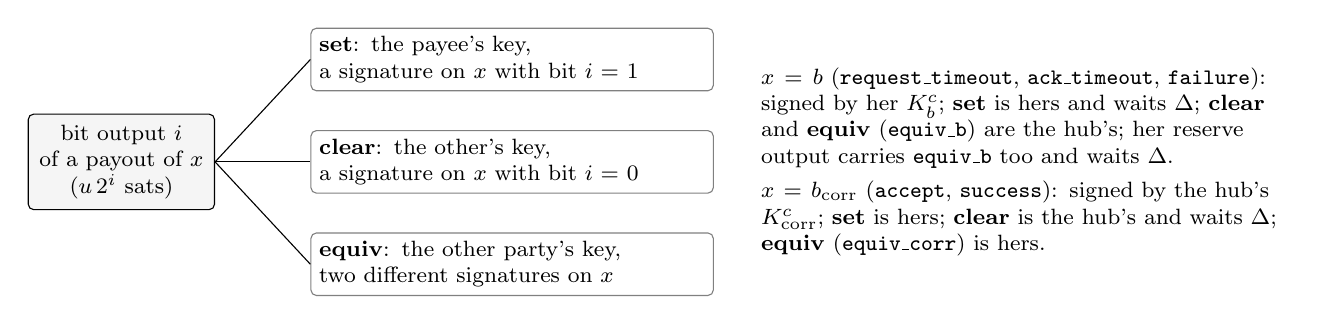
\begin{tikzpicture}[font=\footnotesize,
  bout/.style={draw, rounded corners=2pt, inner sep=4pt, fill=black!4, align=center},
  leaf/.style={draw=black!50, rounded corners=2pt, inner sep=3pt, align=left, text width=4.9cm}]
\node[bout] (o) at (0,0) {bit output $i$\\ of a payout of $x$\\ ($u\,2^i$ sats)};
\node[leaf, anchor=west] (l1) at (2.4, 1.3)  {\textbf{set}: the payee's key,\\ a signature on $x$ with bit $i$ = 1};
\node[leaf, anchor=west] (l2) at (2.4, 0)    {\textbf{clear}: the other's key,\\ a signature on $x$ with bit $i$ = 0};
\node[leaf, anchor=west] (l3) at (2.4, -1.3) {\textbf{equiv}: the other party's key,\\ two different signatures on $x$};
\draw (o.east) -- (l1.west); \draw (o.east) -- (l2.west); \draw (o.east) -- (l3.west);
\node[anchor=west, align=left, text width=6.7cm] at (8.0, 0) {
  $x = b$ (\tx{request\_timeout}, \tx{ack\_timeout}, \tx{failure}): signed by her $\Kb$; \textbf{set} is hers and waits $\Delta$; \textbf{clear} and \textbf{equiv} (\tx{equiv\_b}) are the hub's; her reserve output carries \tx{equiv\_b} too and waits $\Delta$.\\[3pt]
  $x = \bcorr$ (\tx{accept}, \tx{success}): signed by the hub's $\Kcorr$; \textbf{set} is hers; \textbf{clear} is the hub's and waits $\Delta$; \textbf{equiv} (\tx{equiv\_corr}) is hers.};
\end{tikzpicture}
\caption{Above, a contract's graph: solid boxes carry the value on,
dashed ones are terminals; each edge is a pre-signed spend of its
parent's output, with its poster and witness, or its relative
timelock. Below: each bit output of a $\dagger$ terminal's payout, one
per bit position $i$, worth $u\,2^i$ sats. The signer of $x$ waits
$\Delta$, so the other party can show an equivocation first.}
\label{fig:graph}
\end{figure}

\subsection{Bits and equivocation}\label{sec:bits}

A payout of $x$ units (in \tx{request\_timeout}, \tx{accept},
\tx{ack\_timeout}, \tx{success} or \tx{failure}) has, for each bit
position $i$ of the contract, an output of $u\,2^i$ sats. Each is spent
by presenting the one-time signature on $x$ \emph{again}, its leaf
reading bit $i$ from the digits: the payee takes it if the bit is set,
the other party if clear. Whoever signed $x$ could present a signature
on another value, so the other party has a third leaf, taking the
output on two different signatures under that key, and the signer's own
leaf waits $\Delta$ to give it time (Figure~\ref{fig:graph}, below).

This is also why $b$ has its own key, apart from the claim's: each bit
output re-presents $\Wots_{\Kb}(\be{b}{4})$, about 20 witness items;
with $b$ inside the claim's signature, every bit output would verify
some 320.

The one-time keys that sign values the bit outputs don't read ($\KQ$,
$\KU$, $\Acorr$, $\AU$) need no equivocation leaf: a second signature
under one of them has nowhere on chain to do harm. (Off chain it can:
\S\ref{sec:state}.)

\textbf{Windows} on Mutinynet (30\,s blocks): $w_H$ for the hub's moves
(\tx{correct} after \tx{request}; \tx{assert} after \tx{ack}, which must
cover proving: \S\ref{sec:costs}); $w_A$ for her \tx{ack} (2,880 blocks,
a day, as her challenge); $\Delta_2$ = 2,880 for her challenge;
$\Delta_1$ = 240 for the hub's answer.

\textbf{No penalty.} \tx{accept} and \tx{success} return her reserve
whatever $\bcorr$. A false claim gains her nothing (she is paid what she
is owed) and costs the hub one dispute; a penalty would also strike an
honest wallet restored from a stale backup.

\subsection{Withdrawal}\label{sec:withdrawal}

Alice hands the hub her claim (\S\ref{sec:claim}) signed with $a_c$.
The hub takes it if the note is her account's live one: it marks the
account closed, and both sign the fold, which pays her $u\,b$ and $r_A$.
What the note held beyond $u\,b$ the hub issues to her wallet's key with
no contract, as credit. If the hub takes the claim and then won't fold,
she exits with the same note: the account has made no step since, so
the hub has nothing to cite against it.

\section{The exit}\label{sec:exit}

\subsection{The claim}\label{sec:claim}

\begin{definition}
A \emph{claim} on contract $c$ is $(b;\ k, v, \sigma)$: a note of her
account, $(\Oc, k, v)$, with its signature (none for $k = 0$, the mint,
whose value is $v_0$); and $b \le \lfloor v/u \rfloor$.
\end{definition}

An honest wallet claims its live note. If it has a spend in flight, it
still claims the note that spend takes: the step, if the hub uses it,
counts by itself (\S\ref{sec:algo}). The wallet sets $b$ to what she
withdraws.

\textbf{The posted claim} $Q$ is what \tx{request} carries, exactly
$L_Q = 74$ bytes:
\[
  Q = \be{k}{4} \,\|\, \be{v}{6} \,\|\, \sigma^{(64)},
\]
zeros in place of $v$ and $\sigma$ when $k = 0$. The owner, the contract
and $v_0$ are not in $Q$: the statement takes them from the journal.
$b$ is not in $Q$: \tx{request} signs it under its own key
(\S\ref{sec:bits}).

A claim covers the whole balance of the account. There is no subset to
choose and no capacity to exceed.

\textbf{\tx{request}'s witness}: $\Wots_{\KQ}(Q)$ and
$\Wots_{\Kb}(\be{b}{4})$, under the 2-of-2's two signatures: $2(2 \cdot
74 + 3) + 2(8 + 2) + 2 = 324$ stack items, well inside Bitcoin's 1,000.

\subsection{The hub's correction}\label{sec:correct}

\begin{definition}
An exit's \emph{unlock} is $U \in \{0,1\}^{128}$: $U = z_S$ if the hub
cites spend $S$ against the claim, and $U = 0^{16}$ if it cites none.
\end{definition}

The hub posts $U$ in \tx{correct}; the statement derives its scalar $t$
from $U$ by the rule that gives $t_S$ from $z_S$ (\S\ref{sec:grant}).
One seed is always enough (\S\ref{sec:volume}).

When \tx{request} appears, the hub:
\begin{enumerate}[nosep]
\item reads $b$ and $Q$ from \tx{request}'s witness, and looks up the
  account of $\Oc$ in its book;
\item if a recorded spend of the account takes a note at or after the
  claimed one, picks the one that leaves her least: for an honest claim
  this can only be her spend in flight;
\item computes $x = \owed(\cdot)$ (Algorithm~1) with the statement's own
  function, taking as $U$ that spend's seed, or zeros;
\item takes the claim into its book at $x$, in the same step: the
  account is closed, so no later spend of it is recorded;
\item if $x = b$: does nothing, and \tx{request\_timeout} pays $b$;
\item otherwise posts \tx{correct} with $\bcorr = x$ and $U$, each under
  its one-time key: $\Wots_{\Kcorr}(\be{\bcorr}{4})$ and
  $\Wots_{\KU}(U)$.
\end{enumerate}

\subsection{Alice's answer: accept or countersign}\label{sec:ack}

\tx{correct} is public, and so is $U$. If Alice has a spend $(S,
\Gamma)$ in flight and $U$'s seed has the scalar $t$ with $tG = T_S$,
she completes her new note, $\Compl(\rho, t)$, hands $z_S$ to the
counterparty, and drops $S$ from in flight. Then:
\begin{itemize}[nosep]
\item \textbf{Accept}: she does nothing. After $w_A$, \tx{accept} pays
  her $\bcorr$ and $r_A$. No proof.
\item \textbf{Contest}: she posts \tx{ack}, whose leaf verifies
  \[
    \Wots_{\Kcorr}(\be{\bcorr}{4}),\ \Wots_{\Acorr}(\be{\bcorr'}{4}),\
    \Wots_{\KU}(U),\ \Wots_{\AU}(U'),
  \]
  the hub's two signatures copied from \tx{correct} and hers, and checks
  digit by digit that $\bcorr' = \bcorr$ and $U' = U$. Script can do
  this because both signatures' digits are on the stack. So her
  signatures under $\Acorr$ and $\AU$ can only be on the values the hub
  signed.
\end{itemize}
Contesting is mechanical: she signs what she read. She needs no proof,
and will never need one.

\subsection{The hub's statement}\label{sec:statement}

\emph{The claim Alice signed is owed at most the $\bcorr$ she
countersigned.}

\textbf{Private input}: $(\Piss, \Oc, u)$; her four one-time public
keys and the four signatures under them, from \tx{request}'s and
\tx{ack}'s witnesses: $\Wots_{\KQ}(Q)$, $\Wots_{\Kb}(\be{b}{4})$,
$\Wots_{\Acorr}(\be{\bcorr}{4})$ and $\Wots_{\AU}(U)$; $v_0$; and at
most one cited spend
\[
  X = \big(\eta,\ o',\ h',\ T^{(33)},\ \rho_1, \rho_2,\ \psi_1, \psi_2\big):
\]
her half $\eta$ (owner $\Oc$), the other owner and its half's digest,
the grant's point and pre-signatures, and both owners' signatures. From
these the statement recomputes $\delta(S)$, ordering the two owners, and
$\alpha$. The other half stays a digest: the statement never learns the
counterparty's balance.

\textbf{Checks}, in order (any failure rejects; no proof):
\begin{enumerate}[nosep]
\item The keys hash to $\kappa$, and $\be{c}{4} \,\|\, D = J$.
\item The four one-time signatures verify under her keys. Their digits
  give $Q$, $b$, $\bcorr$ and $U$.
\item $\owed(Q, b, \Oc, u, v_0, X, U) \le \bcorr$ (Algorithm~1).
\end{enumerate}
\textbf{Output}: $J$.

\textbf{A number, not a verdict.} $\owed$ returns an amount in units;
the statement's predicate is $\owed \le \bcorr$. The graph pays $b$ or
$\bcorr$, by path (Figure~\ref{fig:exit}): $b$ if the hub stays silent,
doesn't assert, or asserts a false proof; $\bcorr$ if Alice accepts or
the proof stands. Nothing pays 0 as such: the hub posts $\bcorr = 0$,
and can prove it only when $\owed = 0$, for an account she emptied or a
malformed claim.

\textbf{Why she countersigns.} The journal is fixed at the opening,
while $Q$, $b$, $\bcorr$ and $U$ arise at exit, and the statement reads
no chain. Every one of them reaches it under one of \emph{Alice's}
one-time keys, bound in $J$:
\begin{itemize}[nosep]
\item $Q$ and $b$ are hers, signed in \tx{request}: amount
  authentication as in~\cite{lichen}.
\item $\bcorr$ and $U$ are the hub's, the prover's own values. The
  hub's signature can't carry them: the hub could sign one value on
  chain and another for its proof, an equivocation Alice never sees.
  Her countersignature can: script forces it to equal what the hub
  published, and she signs once.
\end{itemize}
This is the countersignature of BABE with authenticated
amounts~\cite{lichen,delving}, with the roles swapped: there the hub
countersigns and Alice proves; here Alice countersigns and the hub
proves. Only the hub ever proves.

\textbf{One-sided suffices.} The statement bounds $\owed$ from above
only, because the hub chooses $\bcorr$ and bears the burden:
\begin{itemize}[nosep]
\item $\bcorr$ too low: the hub can't prove; \tx{ack\_timeout} or
  \tx{failure} pays $b$.
\item $\bcorr$ too high: only the hub loses.
\item No \tx{ack}: she accepted $\bcorr$; no proof.
\item A seed whose scalar doesn't give $T$: the spend doesn't count,
  which hurts only the hub.
\end{itemize}

\subsection{Algorithm 1}\label{sec:algo}

\begin{algobox}{Algorithm 1: $\owed(Q, b, O, u, v_0, X, U)$, in units}
\textbf{Malformed: return 0} if $Q$ doesn't parse; or $k > 0$ and not
$\Vfy_{\Piss}(\delta(O, k, v), \sigma)$; or $b > \lfloor v/u \rfloor$
(with $v = v_0$ if $k = 0$).\\[3pt]
\textbf{Supersedes.} $X$ \emph{supersedes} the claim iff
(a) $\Vfy_{o_i}(\alpha, \psi_i)$ for both owners, one of them $O$, whose
half is $\eta$;
(b) $U \ne 0^{16}$ and $t\,G = T$, $t$ the scalar of $U$; and
(c) $\eta$'s $\kin \ge k$.\\[3pt]
\textbf{Return} $\min(b, \lfloor \vout/u \rfloor)$, $\vout$ from $\eta$,
if $X$ supersedes the claim; else $\min(b, \lfloor v/u \rfloor)$.
\end{algobox}

A cited step of her account at or after the claimed note replaces it:
she is owed what that step left her. Otherwise the claimed note stands.

\textbf{Why $\ge$, and why it is enough.} The statement can't tell
which step is an account's latest: it checks only that the cited one is
real (both signatures, its seed published) and not before the claimed
note. That is enough:
\begin{itemize}[nosep]
\item \textbf{An honest claim leaves the hub no choice.} Claiming her
  live note $k$, the only step she ever signed with $\kin \ge k$ is the
  one in flight, if any (Rule 3). The hub may cite it, publishing its
  seed and completing it for both parties, or not. Either way she is
  owed what she holds.
\item \textbf{A stale claim never pays more than a current one.} Claiming
  an old note, she leaves the hub free to cite any later step it holds,
  and it will cite the least. Her latest step is among them, so she is
  paid at most her current balance. Trying her luck on an old, larger
  balance gains nothing.
\item \textbf{Why not $=$.} With $\kin = k$ only, the one spend that
  could answer a stale claim would be the step that took note $k$,
  whose result might be larger than her balance now. The inequality is
  what lets one citation reach the present.
\end{itemize}
This is close to eltoo~\cite{eltoo}: a later state replaces an earlier
one by its number, with no penalty for publishing an old one. Here the
hub supplies the later state, any it holds; one that keeps only the
latest step per account has only that to cite.

\textbf{A spend in flight needs no naming.} The claim doesn't say which
spends she has in flight, and needn't. Crediting a cited step's result
is safe because anything later also qualifies: if a later step exists,
the hub can cite that instead. A spend in flight is just a step she
signed whose result she hasn't seen.

\textbf{The reissue.} A cancelled spend takes note $k$; the reissue is
note $k + 1$. A claim of the reissue sets the bar at $k + 1$, so the
cancelled spend, completed or not, never supersedes it.

\textbf{Faked evidence only hurts the hub.} A cited spend can only lower
what she is owed to what she signed, and one failing a check is ignored.
So a hub feeding the prover bad data leaves her owed more.

\subsection{How much evidence a claim can need}\label{sec:volume}

\begin{proposition}\label{prop:volume}
Whatever spends the hub holds, citing a single one attains the least
value Algorithm~1 can return for a claim. So $U$'s one seed suffices.
\end{proposition}
\begin{proof}
Algorithm~1 looks at one cited spend and returns either the claimed
value or that spend's $\vout$; the hub cites the spend with the least
$\vout$ among those that supersede the claim, or none.
\end{proof}

\subsection{What each side gets}\label{sec:who}

\begin{proposition}[the honest user]\label{prop:user}
Let Alice claim her live note, and let her one-time keys sign only in
\tx{request} and \tx{ack}. Then she is paid at least $\min(b, \lfloor
x/u \rfloor)$, where $x$ is her note's value, or, if the hub cites her
spend in flight, what that spend left her; and in that case $U$ is its
seed, so the payment completes for both parties.
\end{proposition}
\begin{proof}[Argument]
If she accepts, she is paid $\bcorr$, which she judged; if she contests
and the hub can't prove, $b$. A proof needs her signatures, which exist
only on chain, on the values the hub published: so the statement's $U$
and $\bcorr$ are \tx{correct}'s. A superseding $X$ carries her $\psi$ on
a grant she checked, so it is a step she signed, with $\kin \ge k$; by
Rule 3 that is her spend in flight, and its seed is in $U$, which she
read.
\end{proof}

\begin{proposition}[the hub]\label{prop:hub}
Suppose every spend the hub records satisfies the statement's checks,
it keeps, for each account, the spend that made its live note, and it
posts \tx{correct} within $w_H$ of \tx{request} and \tx{assert} within
$w_H$ of \tx{ack}. Then for any claim on $c$ it pays at most the value
of the account's live note in its book (or what a recorded spend in
flight left her), at most $b$; a malformed claim gets 0.
\end{proposition}
\begin{proof}[Argument]
For each spend it recorded, the hub holds both $\psi$ and derives
$z_S$. A claim of the live note is owed that note, or the spend in
flight if the hub cites it. A stale claim of note $k$ is superseded by
the spend that made the live note, whose $\kin \ge k$: citing it gives
the live value. If Alice accepts, the hub pays its own $\bcorr$; if she
contests, her countersignature is on exactly its values.
\end{proof}

\subsection{State and liveness}\label{sec:state}

\textbf{What each party stores.} Only the latest state of an account.
\begin{itemize}[nosep]
\item \textbf{The user}: the contract's data fixed at the opening (the
  graph's pre-signatures; her one-time and BABE secrets, derivable from
  her seed and the contract's nonce); her live note $(k, v, \sigma)$;
  and at most one spend in flight with its grant.
\item \textbf{The hub}: for each account, its live note, the spend that
  made it (both halves, both signatures, the grant), and any spend in
  flight. Older spends can be dropped once both their accounts have
  moved on. Per contract, the BABE instances it kept at the opening,
  which are bulk but fixed.
\end{itemize}
Nothing grows with history: the hub's storage is $O(1)$ per account,
$O(N)$ for $N$ accounts, whatever the volume of payments. Lightning's
channels keep every revoked state's secrets, because publishing an old
state is punished; here an old state is merely superseded, as in eltoo.
A wallet restored from a backup claims an old note and is paid at most
its current balance, and exactly that if the hub keeps only latest
steps; it should ask the hub for its live note before exiting.

\textbf{Who must be online, and when.} The hub can't move against an
account at all: the graph starts with her \tx{request}, and the hub's
only path is \tx{default} after $\Tc$. So she is online
\begin{itemize}[nosep]
\item to pay or be paid (both parties, for about two round trips);
\item during her own exit, to accept or countersign within $w_A$, with
  keys; she chose when to exit;
\item once per contract, before $\Tc$: to withdraw, exit or roll over.
\end{itemize}
There is nothing to watch for between payments, no hot wallet in
Lightning's sense, and no harm in going offline with a payment in
flight. The hub must be online for payments and for \tx{correct} and
\tx{assert}.

\textbf{When anyone reads the chain.} The chain is a court and a
bulletin board, consulted only when something is stuck. Nothing can be
published against a user: every exit starts with her own \tx{request}.
So a wallet can ignore the chain by default, and reads it in three
cases:
\begin{itemize}[nosep]
\item her own exit, which she started and follows to its end;
\item a stuck incoming payment: the payee asks the payer for $z_S$, and
  failing that finds it in the $U$ of the payer's \tx{correct}. It
  needs no knowledge of the payer's contract: it tests the seed of each
  \tx{correct} the hub posts against $T_S$, one $t\,G$ apiece;
\item the close $\Tc$, which needs a clock, not watching.
\end{itemize}
Only the hub watches continuously, to answer each \tx{request} within
$w_H$. In Lightning the chain is a standing threat, guarded against at
all times; here it is consulted on demand.

\textbf{The countersignature takes keys.} \tx{ack} is signed with
$\Acorr$ and $\AU$. A tower can hold them, but not without trust. On
chain a tower can't misuse them (script forces equality), but off chain
it could sign other values and hand them to the hub, whose proof would
then rest on a $U$ and $\bcorr$ that Alice never saw. Her challenge of
a false proof, by contrast, reveals labels, which a keyless tower can
do.

\section{An exit, step by step}\label{sec:example}

Figure~\ref{fig:exit} shows a contested exit.

\begin{figure}[!tbp]
\centering
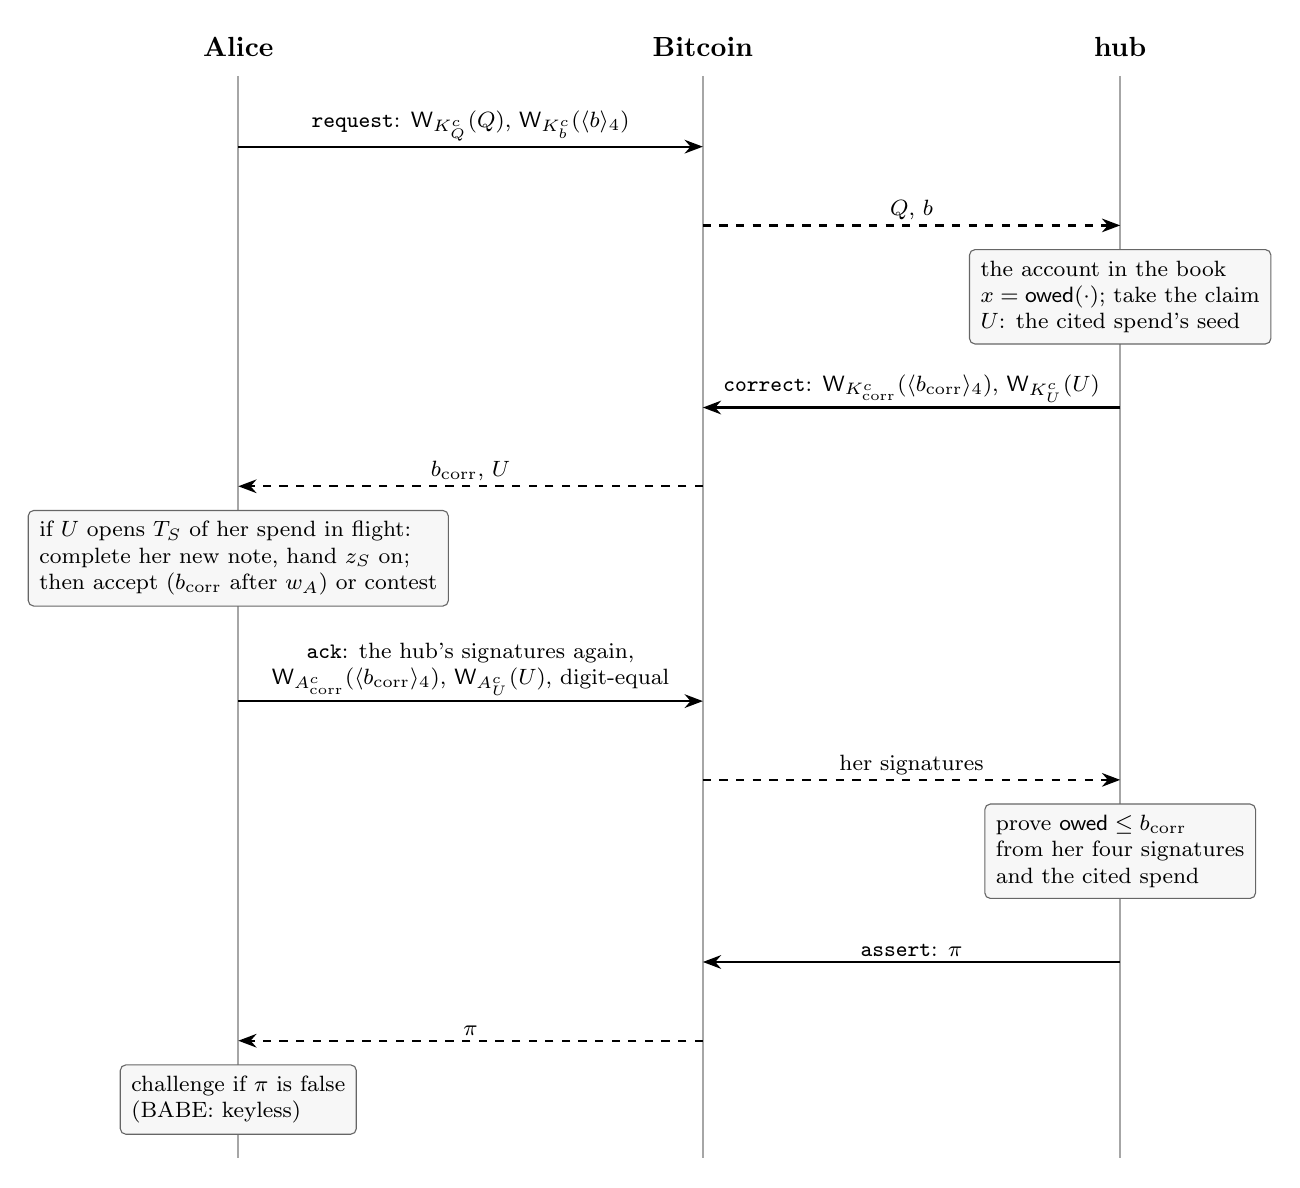
\begin{tikzpicture}[>=Stealth, font=\small,
  life/.style={draw=black!35, thick},
  box/.style={draw=black!60, fill=black!3, rounded corners=2pt, align=left, inner sep=4pt, font=\footnotesize},
  msg/.style={->, thick},
  lbl/.style={align=center, font=\footnotesize, inner sep=1.5pt}]
\coordinate (LA) at (2.6,0); \coordinate (LB) at (8.5,0); \coordinate (LH) at (13.8,0);
\node[font=\bfseries, anchor=base] at ($(LA)+(0,0.25)$) {Alice};
\node[font=\bfseries, anchor=base] at ($(LB)+(0,0.25)$) {Bitcoin};
\node[font=\bfseries, anchor=base] at ($(LH)+(0,0.25)$) {hub};
\coordinate (y) at (0,-0.9);
\draw[msg] (LA|-y) -- node[lbl, above] {\tx{request}: $\Wots_{\KQ}(Q)$, $\Wots_{\Kb}(\be{b}{4})$} (LB|-y);
\coordinate (y) at ($(y)+(0,-1.0)$);
\draw[msg, dashed] (LB|-y) -- node[lbl, above] {$Q$, $b$} (LH|-y);
\node[box, anchor=north] (h1) at ($(LH|-y)+(0,-0.3)$) {the account in the book\\ $x = \owed(\cdot)$; take the claim\\ $U$: the cited spend's seed};
\coordinate (y) at ($(h1.south)+(0,-0.8)$);
\draw[msg] (LH|-y) -- node[lbl, above] {\tx{correct}: $\Wots_{\Kcorr}(\be{\bcorr}{4})$, $\Wots_{\KU}(U)$} (LB|-y);
\coordinate (y) at ($(y)+(0,-1.0)$);
\draw[msg, dashed] (LB|-y) -- node[lbl, above] {$\bcorr$, $U$} (LA|-y);
\node[box, anchor=north] (a1) at ($(LA|-y)+(0,-0.3)$) {if $U$ opens $T_S$ of her spend in flight:\\ complete her new note, hand $z_S$ on;\\ then accept ($\bcorr$ after $w_A$) or contest};
\coordinate (y) at ($(a1.south)+(0,-1.2)$);
\draw[msg] (LA|-y) -- node[lbl, above] {\tx{ack}: the hub's signatures again,\\ $\Wots_{\Acorr}(\be{\bcorr}{4})$, $\Wots_{\AU}(U)$, digit-equal} (LB|-y);
\coordinate (y) at ($(y)+(0,-1.0)$);
\draw[msg, dashed] (LB|-y) -- node[lbl, above] {her signatures} (LH|-y);
\node[box, anchor=north] (h2) at ($(LH|-y)+(0,-0.3)$) {prove $\owed \le \bcorr$\\ from her four signatures\\ and the cited spend};
\coordinate (y) at ($(h2.south)+(0,-0.8)$);
\draw[msg] (LH|-y) -- node[lbl, above] {\tx{assert}: $\pi$} (LB|-y);
\coordinate (y) at ($(y)+(0,-1.0)$);
\draw[msg, dashed] (LB|-y) -- node[lbl, above] {$\pi$} (LA|-y);
\node[box, anchor=north] (a2) at ($(LA|-y)+(0,-0.3)$) {challenge if $\pi$ is false\\ (BABE: keyless)};
\coordinate (end) at ($(a2.south)+(0,-0.3)$);
\begin{scope}[on background layer]
\foreach \l in {LA,LB,LH} \draw[life] (\l) -- (\l|-end);
\end{scope}
\end{tikzpicture}
\caption{A contested exit. Dashed arrows: reading the chain. Silence
ends it: no \tx{correct}, $b$; no \tx{ack}, $\bcorr$; no \tx{assert},
$b$; a valid $\pi$ unchallenged, $\bcorr$; a false one challenged, $b$.}
\label{fig:exit}
\end{figure}

\textbf{A worked example.} Unit $u = 100$ sats. Alice's contract key $O$
holds the note $(O, 5, 100{,}000)$. She pays Bob 50,000: her half is
$(O, 5, 100{,}000, 50{,}000, \lambda_A)$. Both sign; the hub records $S$
but withholds $z_S$, so both are in flight. She exits with $b = 1000$,
claiming note 5.
\begin{itemize}[nosep]
\item The hub is silent: \tx{request\_timeout} pays her 1000 units. Her
  payment to Bob never settled, and he still holds his old note.
\item The hub posts \tx{correct} with $\bcorr = 500$ and $U = z_S$.
  Alice reads $z_S$, completes $(O, 6, 50{,}000)$, and hands $z_S$ to
  Bob, whose new note settles too. $S$ supersedes the claim ($\kin = 5
  \ge 5$), and Algorithm~1 returns $\min(1000, \lfloor
  50{,}000/100\rfloor) = 500$. Whether she accepts or contests, she is
  paid 500 units and $r_A$.
\item The hub posts $\bcorr = 300$: she contests, it can't prove $\owed
  \le 300$, and she is paid 1000.
\item The hub posts $\bcorr = 500$ with a wrong seed in $U$: she
  contests; $S$ doesn't supersede, $\owed = 1000$, and she is paid 1000.
\end{itemize}
Had she claimed an old note, say number 3 of 120,000, the hub would
cite $S$ all the same ($5 \ge 3$), and she would get 500.

\section{Option: deferred receipt}\label{sec:deferred}

The live design asks the payee to be online when paid. A mailbox can
relax that, at a price. Alice signs first; the hub keeps the spend in
Bob's mailbox; Bob signs when he next connects; then the hub releases
$z_S$ to both. Rule 1 already makes this safe in one direction: until
Bob signs, $S$ counts against no one, so Alice can't be debited for a
payment Bob never accepted. What has to be added:

\begin{enumerate}[nosep]
\item \textbf{The hub forms the payee's half.} Bob's half takes his live
  note, which Alice must not see; so the hub writes $\eta_B$, with a
  blinding of its own, and Bob checks it when he signs. A half he finds
  wrong, he refuses.
\item \textbf{One payment per payee in the mailbox.} A second payment to
  Bob would take note $k_B + 1$, which doesn't exist until he signs the
  first. So the hub queues later payers without forming their spends,
  and they sign only when their turn comes: they must be online then,
  or the queue skips them.
\item \textbf{The payer is in flight while the payee is away.} Alice's
  account is held for as long as Bob stays offline, and by Rule 2 she
  can make no other payment. Her wallet cancels after a timeout
  (\S\ref{sec:rules}), and the cancel races Bob's signature: the hub
  serializes them, answering her with $z_S$ if his arrived first.
\item \textbf{Late signatures.} Bob may sign a spend Alice already
  cancelled. The hub refuses it, so Bob is in flight on a spend that
  will never complete and needs a reissue of his own. Every pending
  spend can strand both its parties.
\item \textbf{Settling into a closed contract} (\S\ref{sec:atomic})
  needs longer timeouts: a payment is pending for as long as its payee
  is away, not for a round trip, and $p$ and $L$ must cover it.
\end{enumerate}

None of this changes the exit, the statement or Algorithm~1: the cost is
all in the payment protocol and the wallet's timeouts. The alternative,
letting an offline payee hold several notes and merge them later, is a
different design (\S\ref{sec:compare}).

\section{Costs}\label{sec:costs}

Nothing in this design is built. The dispute graph's shape has been
built and measured on regtest with longer values: a 137-byte claim
(\tx{request} 8,891 vB with 578 stack items) and 64 bytes of unlock
(\tx{correct} 3,611 vB with 284; \tx{ack} 8,025 with 566). The link
sizes below scale those in proportion to stack items. Statement cycles
are from measured parts: a BIP340 verification is about 260k cycles in
RISC Zero, a SHA-256 compression about 490.

\begin{center}
\begin{tabularx}{\linewidth}{lL}
\toprule
Item & Cost (est.) \\
\midrule
\tx{request} & $Q$ (74 bytes) and $b$ under her SHA-256 keys: 324 items, about 5.0 kvB \\
\tx{correct} & $\bcorr$ and $U$ (16 bytes) under the hub's HASH160 keys: $2(8 + 2) + 2(32 + 3) + 2 = 92$ items, about 1.2 kvB \\
\tx{ack} & the hub's signatures again and hers on the same values: 182 items, about 2.6 kvB \\
statement & no headers, no transaction parsing. Her four one-time signatures: about 206 chains, some 1,500 compressions, 0.75M cycles; the note's signature and two $\psi$: 3 BIP340 checks, 0.8M; one $t\,G$, about 0.15M. About 1.7M cycles, 2 segments: proving in a minute or two on a laptop \\
payment & about two round trips for each party; each checks one pre-signature and makes one BIP340 signature \\
hub's book & per account: the live note, the spend that made it, any spend in flight \\
\bottomrule
\end{tabularx}
\end{center}

\textbf{Why a seed.} \tx{ack} carries two one-time signatures on every
byte of $U$, 8 stack items a byte. A 16-byte seed, from which the
statement derives $t$, takes half the items of the 32-byte scalar. The
scalar can't simply be short: with $t < 2^{128}$, the kangaroo method
finds $t$ from $T$ in about $2^{64}$ steps, and anyone holding a grant
could then complete both new notes without the hub publishing anything,
which ends atomicity. Hashing the seed spreads its 16 bytes over a
full-size scalar, so finding $t$ means guessing $z$: $2^{128}$ work.

\textbf{Who pays.} The statement's cost is the hub's alone: only the
hub proves, and only when it corrects a claim and she contests. $w_H$
for \tx{assert} must cover its proving time. The user's costs are a
wallet's: a BIP340 signature and a pre-signature check per payment, and
her moves on chain, \tx{request} and perhaps \tx{ack}.

\section{Payment volume}\label{sec:volume-pay}

Nothing in this design grows with the number of payments. Each payment
replaces one step of each of two accounts: the hub keeps the latest
step, the parties their live notes, and an exit costs the same after
one payment or a billion. The counter is 32 bits, about $4.3 \times
10^9$ payments per account, 50 days at a thousand a second; a contract
closes at $\Tc$ anyway, and a new one starts a new account at 0. So a
pair can stream a million payments of 1 sat each and leave behind
exactly what one payment leaves. Volume over time is unbounded; what
bounds it is the rate.

\textbf{The rate.} A payment is about two round trips for each party,
and Rule~2 allows one pending payment per account. So one pair streams
at about $1/(2\,\mathit{RTT})$: 5--20 payments a second over the
internet, a million in a day or so. The hub's work per payment is two
pre-signatures and two verifications, microseconds; pairs of accounts
that share none don't contend, so the hub can shard its book by
account, a payment locking only the two it touches. Below a unit $u$,
value is lost at exit, not in the L2: the L2 counts sats.

Table~\ref{tab:ln} sets this against Lightning, for the closest
equivalent: a payment from Alice to Bob through one node (an LSP),
Alice $\to N \to$ Bob.

\begin{table}[!tbp]
\centering\small
\renewcommand{\arraystretch}{1.15}
\begin{tabularx}{\linewidth}{>{\raggedright\arraybackslash}p{2.7cm}LL}
\toprule
Per payment & Lightning, through one node & This design \\
\midrule
messages & per hop an add and a fulfil, each a commitment exchange both ways: about 20 & 9 messages; about 2 round trips for each party \\
signatures made & each side, per hop and update, a commitment and its HTLCs: 8 and more & 4: the hub's two pre-signatures and the parties' two $\psi$ \\
signatures verified & as many & 4: the hub two $\psi$, each party one pre-signature \\
kept by the parties & per revoked state, what punishing it takes: secrets compress ($O(\log n)$, shachain), HTLC data doesn't & nothing new: the live note replaces the old \\
kept by the node or hub & the same, per channel & the latest step per account, overwritten \\
kept by a tower & a blob per state & nothing; there is nothing to watch \\
an old state published & punished: all funds to the other side & superseded: paid at most the current balance \\
\midrule
Over time & & \\
\midrule
payments per account & unbounded, at growing storage & unbounded at $O(1)$ storage ($2^{32}$ per contract) \\
in flight per pair & up to 483 HTLCs each way, pipelined & one; more by more accounts, splitting liquidity \\
rate per pair & bounded by bandwidth and compute & about $1/(2\,\mathit{RTT})$, 5--20 a second \\
watching between payments & continuous, or a tower & none \\
\midrule
Around it & & \\
\midrule
who sees a payment & each hop its amount; the onion hides the ends & the hub: both parties and the amount \\
reach & the whole network, without trust & one hub's users \\
fixed cost per user & a channel open; a force close, a few hundred vB & a contract with its BABE setup; an exit, 5--17 kvB \\
\bottomrule
\end{tabularx}
\caption{Payment volume against Lightning. Lightning's figures are for
the BOLT protocol with LN-penalty channels; this design's are
estimates (\S\ref{sec:costs}).}
\label{tab:ln}
\end{table}

\textbf{Where it wins.} Per payment it costs no more than Lightning
through an LSP, and probably less: under half the messages, a handful of
signatures, no commitment transactions, nothing revoked. And nothing
accumulates: a payment channel's history is a liability, kept against an
old state being published; an account's history here is nothing at all.
So very high volumes, streams of small payments, machine-to-machine
metering, are bounded only by how fast two parties and a hub can
exchange nine messages.

\textbf{Where it doesn't.} One pair can't pipeline: Lightning can keep
483 payments in flight on a channel, an account one. The hub sees every
payment and carries all of them; Lightning spreads both. And the reach
is one hub's users.

\section{Against version 0.4: many notes per key}\label{sec:compare}

Version 0.4~\cite{grants04} is the other form of the grants L2. A key
there holds any number of notes, named by 32-byte ids; a payment spends
some of the payer's notes into new ones, and the payee receives offline,
through a mailbox. An exit claims up to four notes, with \emph{fallbacks}
naming spends in flight, and is judged by a fixed point over the set of
claimed notes. Notes are BLS signatures, aggregated so that four fit in
one claim. The exit's graph is the same as here.

\begin{center}
\begin{tabularx}{\linewidth}{lLL}
\toprule
& Version 0.4: many notes & This design: one note per account \\
\midrule
receiving & offline, by mailbox & online, signing (deferred: \S\ref{sec:deferred}) \\
notes per key & any; an exit protects 4 & exactly 1, all of it protected \\
note names & 32-byte ids, 16-byte short ids & (owner, number) \\
merges & needed, and need the hub & none \\
hub's storage & every spend: grows with payments & $O(1)$ per account: $O(N)$ users \\
unclaimable balance & notes beyond a claim's 4 & none \\
claim $Q$ & 137 bytes: 4 notes, fallbacks & 74 bytes: one note \\
unlocks $U$ & 4 seeds, 64 bytes & 1 seed, 16 bytes \\
\tx{request}, \tx{correct}, \tx{ack} & 8.9, 3.6, 8.0 kvB (measured) & 5.0, 1.2, 2.6 kvB (scaled) \\
Algorithm~1 & fixed point over a set; revivals by named prefix & one comparison of numbers \\
spend in flight & named as a fallback & counts by its number \\
stale claim & 0, if the hub cites what took it & at most the current balance \\
note signatures & BLS, aggregated; encrypted under $T$ & BIP340; adaptor pre-signatures \\
statement & about 29M cycles (a pairing) & about 1.7M (no pairing) \\
concurrency & up to 3 spends in flight & one pending signature per account \\
atomicity & one-way: the payer's side & both sides, the same way \\
counterparty learns & the payee nothing of her change & the amount only (halves) \\
\bottomrule
\end{tabularx}
\end{center}

\textbf{Simpler.} This design has no fixed point and no capacity
argument; the claim has no list and no fallbacks; notes have no ids; the
wallet has no merge policy and no choice of what to claim; and the
statement has no pairing, 1.7M cycles against 29M, half an hour of
proving on a laptop. And since every balance is claimable in full, a
hub that stops serving gains nothing; in version 0.4 it keeps whatever
notes users hold beyond a claim's four.

\textbf{What it costs.} Payees must be online when paid, and an account
makes one payment at a time. These are Lightning's terms for a payee,
without channels or routes, and without Lightning's standing duties:
no watching between payments, and no history to back up.

\textbf{Scaling.} The hub's storage is $O(1)$ per account, $O(N)$ in
all, independent of the number of payments; per payment it does a
constant amount of work; accounts don't contend except pairwise, so
payments between disjoint pairs need no coordination; and an exit costs
the same however long the account's history.

\textbf{The private variant.} One note per account needs arbitrary
values, so it doesn't combine with fixed-denomination ecash, where a
balance takes as many notes as its value has set bits. A private form
would hide amounts and numbers: keyed-verification credentials with
attributes, as in WabiSabi, whose verification key the journal would
have to commit to.

\section{Open questions}\label{sec:open}

\begin{itemize}[nosep]
\item \textbf{Settling into a closed contract} (\S\ref{sec:atomic}):
  wallet timeouts close it in practice. Could the statement bind a
  spend's use to the payee's contract being open, with no timeouts?
\item \textbf{A keyless contest.} \tx{ack} needs her keys within $w_A$
  (\S\ref{sec:state}). Can a tower countersign without being able to
  sign other values off chain?
\item \textbf{Latency of a payment}: two round trips with both parties
  online. How does a phone answer an incoming payment in the background?
\item \textbf{Fees}: a third half, the hub's own account, or a part of
  the payer's.
\item \textbf{Rules at exit.} The statement could enforce predicates
  fixed at the opening: a cited spend supersedes only if it meets them.
  Like everything here, they limit only what the hub can debit; they
  bind the two parties to the contract and no one else; and they have
  no clock but the chain's. One example is a floor $F$: spending below
  it needs a second, cold key, aggregated with the first (MuSig2), so
  the statement still checks one signature. It helps only if her key is
  stolen. The hub may ignore the rule and pay the thief, but it can't
  debit her for it.
\item \textbf{Measurement}: the statement's cycles and the links' sizes
  are estimates from measured parts.
\end{itemize}

\begin{thebibliography}{9}
\bibitem{lichen} waxwing, \emph{Lichen}, version 0.5, 2026.
\bibitem{grants04} waxwing, \emph{The grants L2: the countersigned exit,
  with BLS notes}, version 0.4, November 2026.
\bibitem{delving} waxwing, \emph{Variable payout amounts for BABE, as
  applied to Lichen}, Delving Bitcoin, October 2026.
\bibitem{bip340} P.~Wuille, J.~Nick, T.~Ruffing, \emph{BIP 340: Schnorr
  signatures for secp256k1}, 2020.
\bibitem{poelstra} A.~Poelstra, \emph{Scriptless scripts}, 2017.
\bibitem{aumayr} L.~Aumayr, O.~Ersoy, A.~Erwig, S.~Faust,
  K.~Hostáková, M.~Maffei, P.~Moreno-Sanchez, S.~Riahi,
  \emph{Generalized channels from limited blockchain scripts and
  adaptor signatures}, ASIACRYPT 2021.
\bibitem{eltoo} C.~Decker, R.~Russell, O.~Osuntokun, \emph{eltoo: a
  simple layer2 protocol for Bitcoin}, 2018.
\end{thebibliography}

\end{document}
